\documentclass[a4paper,11pt]{article}
\usepackage{luatex85}
\usepackage[babelshorthands]{polyglossia}
\usepackage[fleqn,reqno]{amsmath}
\usepackage{amsthm}
\RequirePackage[
	backend=biber,
	bibstyle=gost-numeric,
	citestyle=gost-numeric,
	%defernumbers=true,
	defernumbers=false,
	language=auto,
	autolang=langname,
	]{biblatex}
\usepackage[math-style=ISO,bold-style=upright,partial=italic]{unicode-math}
\usepackage{microtype}
\usepackage[width=16cm,height=24cm]{geometry}
\usepackage[russian]{hyperref}
\usepackage{graphicx}
\usepackage{caption}

\setmainlanguage{russian}

\setmainfont{Cambria}
\setsansfont{Calibri}
\setmonofont{Source Code Pro}[Scale=MatchLowercase]
\setmonofont{Source Code Pro}[Scale=MatchLowercase]
\setmathfont{Cambria Math}[sans-style=literal]
\setmathfont{XITS Math}[range={\mathscr}]

%\addbibresource{\jobname.bib}

\makeatletter

\allowdisplaybreaks[4]

\def\[#1\]{\begin{align*}#1\end{align*}}
\newcommand\eqtag[1]{\refstepcounter{equation}\tag{\theequation}\label{#1}}

%\newcommand\slashfrac[2]{{#1\fracslash#2}}
\newcommand\slashfrac[2]{{#1/#2}}

\newcommand\pr{\operatorname{\textbf{\textup{pr}}}}

\theoremstyle{definition}
\newtheorem{theorem}{Теорема}
\newtheorem*{theorem*}{Теорема}
\newtheorem{lemma}{Лемма}
\newtheorem{definition}{Определение}
\newtheorem{example}{Пример}
%\newtheorem{proof}{Доказательство}

\newcommand\metasetup{\hypersetup{
	pdftitle=\@title,
	pdfauthor=\@author,
	linkbordercolor={0 .5 .25},
	}}

\setlength\overfullrule{5pt}

\makeatother

\begin{document}

\hyphenation{Ла-гран-жа ла-гран-же-вой}

\title{Пара слов о~преобразовании Лежандра}
\author{А.~Н.~Швец}

\metasetup
\maketitle

Преобразование Лежандра, знакомое нам в~связи с~методом Рауса и уравнениями
Гамильтона, является ярким примером преобразования, в~которое вовлечены не
только независимые и~зависимые переменные, но и~первые производные (такие
преобразования называются \emph{контактными}).

Пусть $u(x_1,\ldots,x_n)$~— гладкая функция своих аргументов,
$p_i=\slashfrac{\partial u}{\partial x_i}$. Осуществим переход от букв
$(x,u,p)$ к~новым буквам $(\hat x,\hat u,\hat p)$ по формулам
	\[
	\hat x_i=p_i,
	\quad
	\hat u=\sum_{i=1}^np_ix_i-u,
	\quad
	\hat p_i=x_i.
	\eqtag{eq:legendre}
	\]
Это и есть преобразование Лежандра. Хорошо видно, что преобразование является
инволюцией.

Заметим, что переменные $(x,u,p)$ не являются вполне независимыми. Они
независимы \emph{функционально,} (между ними нет функционального соотношения),
однако зависимы \emph{дифференциально\/}~— имеется соотношение с~участием их
дифференциалов. Внешняя форма Пфаффа обращается для них в~ноль:
	\[
	du-\sum_{i=1}^np_i\,dx_i=0.
	\eqtag{eq:pfaff}
	\]

Преобразования в~пространстве независимых, зависимых переменных и~первых
производных (\emph{пространстве 1"=струй\/} функции $u$) только тогда будут
осмысленными, если они сохраняют соотношение Пфаффа, то есть в~новых переменных
также должно выполняться $\hat p_i=\slashfrac{\partial\hat u}{\partial\hat x_i}$.

Для преобразования Лежандра это так. Действительно,
с~учётом~\eqref{eq:legendre}
	\[
	d\hat u-\sum_{i=0}^n\hat p_i\,d\hat x_i
		=\sum_{i=1}^n(p_i\,dx_i+x_i\,dp_i)-du-\sum_{i=1}^nx_i\,dp_i
		=\sum_{i=1}^np_i\,dx_i-du,
	\]
что равно нулю в~силу~\eqref{eq:pfaff}.

\bigskip

\begin{figure}
\centering
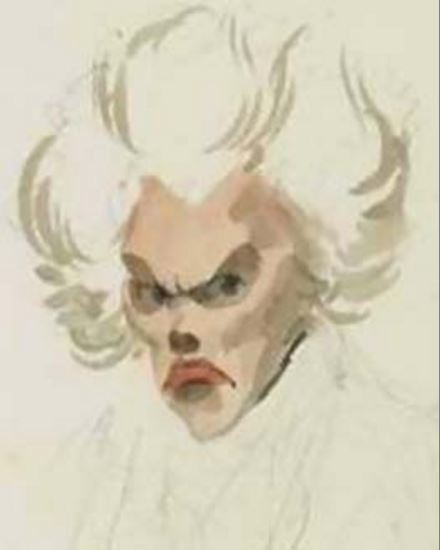
\includegraphics[height=2.5in]{Legendre.png}
\medskip
\caption*{Adrien-Marie Legendre}
% https://en.wikipedia.org/
\end{figure}

Преобразование Лежандра можно использовать для решения обыкновенных
дифференциальных уравнений Клеро (и~для упрощения уравнений других типов)
	\[
	\Phi(p,xp-u)=0,
	\eqtag{eq:clairaut}
	\]
где $p=u'$. После выполнения преобразования Лежандра в~новых переменных получим
	\[
	\Phi(\hat x,\hat u)=0,
	\eqtag{eq:clairaut-trans}
	\]
уравнение отнюдь не дифференциальное. Разрешив его относительно $\hat u$,
получим $\hat u=\varphi(\hat x)$, и, после возврата к~прежним переменным,
получим
	\[
	xp-u=\varphi(p)
	\quad
	\text{или}
	\quad
	u=xp-\varphi(p).
	\]
Мы получили однопараметрическое семейство решений, в~котором в~качестве
параметра выступает~$p=u'$. Решения~$u(x)$ являются аффинными функциями
относительно~$x$, их графики~— прямые. Помимо семейства аффинных функций, среди
решений может появиться особое, его график является огибающей семейства прямых.
Его можно найти, исключив $p$ из уравнений
	\[
	\Phi=0,
	\quad
	\frac{d\Phi}{dp}=0
	\]
(это стандартный способ нахождения огибающих семейства кривых, заданных
неявно). Или, как вариант, можно из указанных уравнений получить выражения
	\[
	x=\alpha(p),
	\quad
	u=\beta(p).
	\]
Это параметрическое представление особого решения, где график запараметризован
$p$~— тангенсом угла наклона. Эта параметризация корректна на участках
выпуклости графика, когда вдоль кривой $p$ меняется монотонно. Особое решение
как раз отвечает случаю, когда уравнение \eqref{eq:clairaut-trans} нельзя
разрешить относительно $\hat x=p$. Для неособых решений, конечно, такая
параметризация неуместна.

\end{document}
